\documentclass[a4paper, 10pt]{article}
% (1) Encoding, Fonts, and Layout
\usepackage[T1]{fontenc}
\usepackage{lmodern}
\usepackage[margin=1in]{geometry}


% (2) Common Packages
\usepackage{amsmath, amssymb, amsthm}
\usepackage{xcolor}
\usepackage{caption}
\usepackage{tikz}
\usepackage{pgfplots}
\pgfplotsset{compat=newest}
\usepackage{etoolbox}
\usepackage{tikz-3dplot}
\tdplotsetmaincoords{75}{120}
\usepackage[inline]{enumitem}
\usepackage{bookmark}
\usepackage{mathtools}
\usepackage{subcaption} 
\usepackage[normalem]{ulem}
\usepackage{booktabs,tabularx}
\usepackage{cleveref}
\usepackage[T1]{fontenc}
\usepackage{xcolor}
\usepackage{fontawesome5}
\usepackage{babel}

\usepackage{minted}
\usepackage[most]{tcolorbox}
\tcbuselibrary{theorems}
\tcbuselibrary{listingsutf8, skins}
\usepackage{microtype}

% Patching pgfplots warning
\makeatletter
\patchcmd{\pgfplots@applistXXpushback@smallbuf}{\pgfplots@error}{\pgfplots@warning}{}{}
\makeatother


\definecolor{custom_green}{HTML}{a3be8c}
\definecolor{custom_red}{HTML}{dc322f}
\definecolor{custom_blue}{HTML}{268bd2}
\definecolor{custom_purple}{HTML}{b48ead}

\definecolor{base}{HTML}{eceff4}
\definecolor{gray1}{HTML}{f8f9fa}
\definecolor{gray2}{HTML}{e9ecef}
\definecolor{gray3}{HTML}{2e3440}
\definecolor{off-white}{HTML}{f4f4f6}


% (5) Custom tcolorbox Environments
\newtcbtheorem[number within=section]{definitionbox}{Definition}{%
    enhanced,
    sharp corners,
    attach boxed title to top left={yshift=-0.1mm},
    colback=custom_red!10,
    colframe=custom_red,
    fonttitle=\bfseries,
    boxed title style={
            sharp corners,
            size=small,
            colback=custom_red,
            colframe=custom_red,
        },
    % Put (#1) after the definition number if a name is given
    description delimiters none,
    % Add a line to the ToC whenever the environment begins
    before upper={%
            \addcontentsline{toc}{subsection}{%
                Definition \thetcbcounter\ifstrempty{#1}{}{#1}%
            }%
        }%
}{def}





\newtcolorbox{conceptbox}[1][]{
    title={#1},
    fonttitle=\bfseries\color{white},
    attach boxed title to top left={yshift=-2mm},
    colbacktitle=custom_blue,
    coltitle=white,
    colframe=custom_blue,
    colback=custom_blue!10,
    boxrule=1mm,
    arc=0mm,
    bottomtitle=0.5mm,
    left=2.5mm,
    leftrule=1mm,
    right=3.5mm,
    rightrule=1mm,
    toptitle=1mm,
    enhanced
}

\lstdefinestyle{cStyle}{
    language=C,
    columns=fullflexible,
    tabsize=4,
    keepspaces=true,
    showstringspaces=false,
    numbersep=5pt,
    numbers=left,
    stepnumber=1,
    basicstyle=\ttfamily\small,
    keywordstyle=\bfseries\color{keywordsblue},
    commentstyle=\itshape\color{commentgreen},
    stringstyle=\color{stringspurple},
    frame=none,
    breaklines=true,
    xleftmargin=0.5em,
}

\newtcblisting{codeexample}[2][]{
    listing only,                        
    title=\emph{Example Code:}\quad  \textbf{#2},         
    fonttitle=\bfseries\scriptsize\color{white},
    attach boxed title to top center={yshift=-1.5mm},
    colbacktitle=custom_green,
    coltitle=white,
    colframe=custom_red,
    colback=custom_red!10,
    boxrule=0.5mm,
    arc=0mm,
    bottomtitle=0.5mm,
    left=2.5mm,
    leftrule=0.5mm,
    right=3.5mm,
    rightrule=0.5mm,
    toptitle=1mm,
    enhanced,
    listing options={style=cStyle} 
}



\newtcolorbox{proofbox}[1][]{
    title=\textbf{Proof:} {#1},
    fonttitle=\bfseries\boldmath,
    arc=0mm,
    bottomtitle=0.5mm,
    boxrule=0mm,
    colbacktitle=gray2,
    colback=gray1,
    coltitle=gray3,
    left=2.5mm,
    leftrule=1mm,
    rightrule=1mm,
    right=3.5mm,
    toptitle=0.75mm,
    colframe=custom_blue,
    coltext=gray3,
}

\newtcolorbox{theorembox}[1][]{
    title=\textbf{Theorem} {#1},
    fonttitle=\bfseries\boldmath,
    arc=0mm,
    bottomtitle=0.5mm,
    boxrule=0mm,
    colbacktitle=gray2,
    colback=gray1,
    coltitle=gray3,
    left=2.5mm,
    leftrule=1mm,
    rightrule=1mm,
    right=3.5mm,
    toptitle=0.75mm,
    colframe=custom_green,
    coltext=gray3
}

\newtcolorbox{notebox}{
    title=\textbf{Note},
    fonttitle=\bfseries\boldmath,
    arc=0mm,
    bottomtitle=0.5mm,
    boxrule=0mm,
    colbacktitle=gray2,
    coltitle=gray3,
    left=2.5mm,
    leftrule=1mm,
    rightrule=1mm,
    right=3.5mm,
    toptitle=0.75mm,
    colframe=custom_blue,
    coltext=gray3
}

% \newtcolorbox{examplebox}[1][]{
%     title=\textbf{Example} {#1},
%     fonttitle=\bfseries\boldmath,
%     arc=0mm,
%     bottomtitle=0.5mm,
%     boxrule=0mm,
%     colbacktitle=gray2,
%     colback=gray1,
%     coltitle=gray3,
%     left=2.5mm,
%     leftrule=1mm,
%     rightrule=1mm,
%     right=3.5mm,
%     toptitle=0.75mm,
%     colframe=gray3,
%     fontupper=\footnotesize,
%     coltext=gray3
% }

\newtcbtheorem[number within=section]{examplebox}{Example}{
    enhanced,
    sharp corners,
    attach boxed title to top left={yshift=-0.1mm},
    colback=gray3!10,
    colframe=gray3,
    colbacktitle=gray2,
    fonttitle=\bfseries,
    boxed title style={
            sharp corners,
            size=small,
            colback=gray3,
            colframe=gray3,
        },
    % Put (#1) after the definition number if a name is given
    description delimiters none,
    % Add a line to the ToC whenever the environment begins
    before upper={%
            \addcontentsline{toc}{subsection}{%
                Example \thetcbcounter\ifstrempty{#1}{}{#1}%
            }%
        }%
}{ex}


\theoremstyle{definition}
\newtheorem{definition}{Definition}[section]
\newtheorem{example}[definition]{Example}

\theoremstyle{plain}
\newtheorem{theorem}[definition]{Theorem}

% (7) Hyperlinks
\usepackage{hyperref}
\hypersetup{
    colorlinks=true,    
    linkcolor=black,      
    pdfborder={0 0 0}   
}


% macros.tex
\newcommand{\intinf}{\int_0^{\infty}} % Integral from 0 to infinity
\newcommand{\diff}[2]{\frac{d#1}{d#2}} % Derivative



% Title and author
\title{
Robert Davidson \\
\textbf{MP232: Applied Mathematics}
}
\author{
60\% Exam\\
40\% Continuous Assessment (3 parts)
}
\date{} % Empty date

\begin{document}
\color{gray3}
\maketitle

\tableofcontents

\pagebreak



\section{Prelim : The Exponential Function and Hyperbolic Functions}
\subsection{Exponential Function}
\noindent \begin{minipage}{0.45\textwidth}
  \textbf{Derivative}
  $$\frac{d}{dt}\bigl(e^{at}\bigr) = a\,e^{at}$$
\end{minipage}\hfill
\noindent \begin{minipage}{0.45\textwidth}
  \textbf{Integral}
  $$\int e^{at}\,dt = \frac{1}{a}e^{at} + C$$
\end{minipage}\hfill



\subsection{Hyperbolic Functions}

\textbf{Definitions:}
$$
  \begin{array}{c | c | c}
    \sinh(at) = \frac{e^{at} - e^{-at}}{2}
     &
    \cosh(at) = \frac{e^{at} + e^{-at}}{2}
     &
    \tanh(at) = \frac{\sinh(at)}{\cosh(at)}.
  \end{array}
$$
\textbf{Derivatives}
$$
  \begin{array}{c | c | c}
    \frac{d}{dt}\bigl(\sinh(at)\bigr) = a\,\cosh(at),
     &
    \frac{d}{dt}\bigl(\cosh(at)\bigr) = a\,\sinh(at),
     &
    \frac{d}{dt}\bigl(\tanh(at)\bigr) = a\,\mathrm{sech}^2(at).
  \end{array}
$$
\textbf{Integrals}
\begin{align*}
  \int \sinh(at)\,dt & = \frac{1}{a}\cosh(at) + C                 \\
  \int \cosh(at)\,dt & = \frac{1}{a}\sinh(at) + C,                \\
  \int \tanh(at)\,dt & = \frac{1}{a}\ln\bigl|\cosh(at)\bigr| + C. \\
\end{align*}
\textbf{Common Identities}
\begin{align*}
  \cosh^2 x - \sinh^2 x & = 1,                                \\
  \sinh(2x)             & = 2\,\sinh x\,\cosh x,              \\
  \cosh(2x)             & = \cosh^2 x + \sinh^2 x,            \\
  \tanh(2x)             & = \frac{2\,\tanh x}{1 + \tanh^2 x}.
\end{align*}

\subsection{Partial Fraction Decomposition}
\textbf{Unrepeated Linear Factors}: A linear factor is of form $(ax + b)$
$$\frac{s + 1}{s(s-2)(s+3)} = \frac{A}{s} + \frac{B}{s-2} + \frac{C}{s+3}$$
\textbf{Repeated LinearFactors}:
$$\frac{3}{(s+2)^2(s-3)} = \frac{A}{s+2} + \frac{B}{(s+2)^2} + \frac{C}{s-3}$$
\textbf{Unrepeated Quadratic Factors with complex roots}: Where the discriminant ($b^2 - 4ac$) is \\
\indent negative (complex roots) but the factor is not repeated
$$\frac{3}{(s^2 - s + 1)(s+2)} = \frac{As + B}{s^2 - s + 1} + \frac{C}{s+2}$$
\textbf{Repeated Quadratic Factors with complex roots}:
$$\frac{1}{(s^2 + 1)^2 (s-1)} = \frac{As + B}{(s^2 + 1)^2} + \frac{Cs + D}{s^2 + 1} + \frac{E}{s-1}$$


\pagebreak
\section{Intro to Laplace Transforms}
\subsection{What is a Laplace Transform?}
\begin{definitionbox}
  The Laplace Transform, defined for $t \geq 0$, is given by
  $$L\{f(t)\}(s) = F(s) = \int_0^\infty e^{-st} dt$$

\end{definitionbox}

\subsection{Common Laplace Transforms}

\begin{examplebox}[Find the Laplace Transform of \boldmath$f(t) = 1$]
  We have:
  $$L\{1\} = \int_0^\infty 1 \cdot e^{-st } dt = \lim_{R \to \infty} \int_0^R e^{-st} dt$$
  This integral is equal to:
  $$\int_0^R e^{-st} dt = \left . \frac{e^{-st}}{-s}\right |_{t=0}^{t=R}
    = -\frac{1}{s}[e^{-sR} - 1] = \frac{1 - e^{-sR}}{s}$$
  Taking the limit as $R \to \infty$ gives:
  $$L\{1\} = \lim_{R \to \infty} \frac{1 - e^{-sR}}{s} = \frac{1}{s}$$
\end{examplebox}

\begin{examplebox}[ Find the Laplace Transform of $f(t) = e^{2t}$]
  \begin{align*}
    L\{e^{2t}\}
     & = \int_0^\infty e^{2t}e^{-st}\, dt
    = \int_0^\infty e^{-(s-2)t}\, dt                                                                               \\[1mm]
     & = \lim_{R\to\infty} \int_0^R e^{-(s-2)t}\, dt                                                               \\[1mm]
     & = \lim_{R\to\infty} \left[ \frac{e^{-(s-2)t}}{-(s-2)} \right]_{t=0}^{t=R}                                   \\[1mm]
     & = \lim_{R\to\infty} \left( \frac{e^{-(s-2)R} - e^0}{-(s-2)} \right)
    = \lim_{R\to\infty} \left( \frac{e^{-(s-2)R} - 1}{-(s-2)} \right)                                              \\[1mm]
     & = \frac{1}{s-2} \quad \text{(since } e^{-(s-2)R} \to 0 \text{ as } R\to\infty \text{ provided } s>2\text{)}
  \end{align*}
\end{examplebox}

\begin{examplebox}[Find the Laplace Transform of $f(t) = \cosh(at)$]
  We have:
  \begin{align*}
    L\{\cosh(at)\} & = L\left\{ \frac{e^{at} + e^{-at}}{2}\right\} \quad \text{from the definition of }\cosh(at)           \\
                   & = \frac{1}{2}L\{e^{at}\} + \frac{1}{2}L\{e^{-at}\} \quad \text{by linearity of the Laplace Transform} \\
                   & = \frac{1}{2}\left(\frac{1}{s-a}\right) + \frac{1}{2}\left(\frac{1}{s+a}\right)
  \end{align*}
  Hence:
  $$L\{\cosh(at)\} = \frac{s}{s^2 - a^2}$$
  Noting that $\sinh(at) = (e^{at} - e^{-at})/2$, we can find that:
  $$L\{\sinh(at)\} = \frac{a}{(s^2 - a^2)}$$
\end{examplebox}

\begin{examplebox}[Find the Laplace Transform of $\cos(wt)$ and $\sin(wt)$ where $w$ is a constant.]
  We first compute the Laplace Transform of $e^{iwt}$ using its definition:
  \[
    L\{e^{iwt}\} = \int_0^\infty e^{-st}e^{iwt}\,dt
    = \int_0^\infty e^{-(s-iw)t}\,dt
    = \frac{1}{s-iw}, \quad \text{for } \Re(s) > 0.
  \]

  To express this in terms of real and imaginary parts, we multiply the numerator and denominator by the complex conjugate of the denominator:
  \[
    \frac{1}{s-iw} = \frac{s+iw}{(s-iw)(s+iw)} = \frac{s+iw}{s^2 + w^2}.
  \]

  Since Euler's formula gives:
  \[
    e^{iwt} = \cos(wt) + i\sin(wt),
  \]
  the linearity of the Laplace Transform yields:
  \[
    L\{e^{iwt}\} = L\{\cos(wt)\} + iL\{\sin(wt)\}.
  \]

  Equating the two representations of $L\{e^{iwt}\}$, we have:
  \[
    L\{\cos(wt)\} + iL\{\sin(wt)\} = \frac{s+iw}{s^2+w^2}.
  \]

  Since the equality must hold for both the real and imaginary parts, we equate them separately:
  \[
    L\{\cos(wt)\} = \frac{s}{s^2+w^2} \quad \text{and} \quad L\{\sin(wt)\} = \frac{w}{s^2+w^2}.
  \]
\end{examplebox}

\subsection{Linearity of the Laplace Transform}
The Laplace Transform is a linear operator, i.e. for any constants $a$ and $b$:
$$L\{af(t) + bg(t)\} = aL\{f(t)\} + bL\{g(t)\}$$
\begin{proofbox}
  \begin{align*}
    L\{af(t) + bg(t)\}
     & = \int_0^\infty e^{-st}(af(t) + bg(t))\, dt                         \\
     & = a\int_0^\infty e^{-st}f(t)\, dt + b\int_0^\infty e^{-st}g(t)\, dt \\
     & = aL\{f(t)\} + bL\{g(t)\}
  \end{align*}
\end{proofbox}

\subsection{The First Shift Theorem}
\begin{theorembox}[First Shift Theorem]
  If $f(t)$ has a Laplace Transform, $F(s)$, defined for $s > k$, then $e^{at}\ f(t)$ has a Laplace Transform, \\ $F(s-a)$ defined for $s - a > k$ and is given by:
  $$L\{e^{at} f(t)\} = F(s-a)$$
  or, taking the inverse Laplace Transform of both sides:
  $$e^{at}f(t) = L^{-1}\{F(s-a)\}$$
\end{theorembox}
\subsubsection{Examples}
\begin{examplebox}[Find the Laplace Transform of $e^{at}\cos(wt)$, where $a,w$ are constants.]
  We know that $L\{\cos(wt)\} = \frac{s}{s^2 + w^2}$, so by the First Shift Theorem:
  \begin{align*}
    L\{e^{at}\cos(wt)\} & = \frac{s-a}{(s-a)^2 + w^2}         \\
                        & = \frac{s-a}{s^2 - 2as + a^2 + w^2}
  \end{align*}
\end{examplebox}
\subsection{Existence of the Laplace Transform}
Existence of a Laplace transform is not always guaranteed because we're integrating over an infinite integral. For a Laplace Transform to exist for a given $s$, then the integral must exist:
$$\int_0^\infty e^{-st}f(t)\, dt$$

\begin{theorembox}[Existence Theorem of Laplace Transforms]
  Suppose $f(t)$ is a piecewise continuous function on $[0,\infty)$. If $f(t)$ satisfies:
  $$|f(t)| \leq Me^{kt} \; (0 \leq t \leq \infty)$$
  for some constants, $M, k$, then the Laplace Transform of $f(t)$ exists for $s > k$. In other words, the Laplace Transform of $f(t)$ exists if $f(t)$ is bounded by an exponential function.
\end{theorembox}

\begin{proofbox}
  If $s > k$, then from the equation above, we have:
  $$|F(s)| = \left | \int_0^\infty f(t)e^{-st} \; dt  \right | \leq \int_{0}^{\infty} |f(t)| e^{-st} \; dt \leq \int_{0}^\infty Me^{(k-s)t} \; dt = \frac{M}{s-k}$$
\end{proofbox}

\section{Applications of Laplace Transforms}
\subsection{Integration by Parts}
Starting with the product rule:
$$
  \frac{d}{dx}[uv] = u'v + uv',
$$
we can express this in differential form as:
$$
  d\bigl(uv\bigr) = u\,dv + v\,du.
$$
Integrate both sides with respect to \(x\):
$$
  \int d\bigl(uv\bigr) = \int_a^b u\,dv + \int_a^b v\,du.
$$
The Fundamental Theorem of Calculus tells us that the left-hand side is simply:
$$
  uv = \int_a^b u\,dv + \int_a^b v\,du.
$$
Rearrange to solve for the desired integral:
$$
  \int_a^b u\,dv = uv - \int_a^b v\,du,
$$

\subsubsection{Examples}

\begin{examplebox}[Use integration by parts to find the Laplace of $f(t) = t$]
  $$L\{t\} = \int_0^\infty te^{-st} \ dt$$
  We integrate by parts by setting:
  $$u = t, \quad dv = e^{-st}, \quad du = 1, \quad v = -\frac{e^{-st}}{s}$$
  Then intengrating by parts gives:
  \begin{align*}
    L\{t\} & = \left [ -\frac{te^{-st}}{s} \right ]_0^\infty + \frac{1}{s}\int_0^\infty e^{-st} \ dt \\
           & = 0 + \frac{1}{s}\left [ -\frac{e^{-st}}{s} \right ]_0^\infty
  \end{align*}
  Hence:
  $$L\{t\} = \frac{1}{s^2}$$
\end{examplebox}

\begin{examplebox}[Use integration by parts to find the Laplace of $f(t) = \cos(t)$]
  Let:
  $$u = e^{-st}, \quad du = -se^{-st}, \quad dv = \cos(t), \quad v = \sin(t)$$
  Then:
  $$
    \intinf e^{-st} \cos(t)\; dt = \left[ e^{-st} \sin(t) \right]_0^\infty + \intinf \sin(t)\cdot se^{-st} dt = 0 + s\intinf e^{-st} \sin(t) dt
  $$
  Considering the $\sin$ part :
  $$u = e^{-st}, \quad du = -se^{-st}, \quad dv = \sin(t), \quad v = -\cos(t)$$
  $$\intinf e^{-st} \sin(t)\ dt = 1 - s \intinf e^{-st} \cos(t) \ dt$$
  Substituting this back into the original integral gives:
  $$
    \intinf e^{-st} \cos(t)\; dt = 1 - s\intinf e^{-st} \cos(t)\ dt = s - s^2\intinf e^{-st} \cos(t)\ dt \\
  $$

  $$L\{cos(t)\}= \dfrac{s}{1+s^2}$$
\end{examplebox}

\subsection{Table of Laplace Transforms}
\renewcommand{\arraystretch}{1.5} % Increase vertical spacing in the table
\small$$
  \begin{array}{|c|c|}
    \hline
    f(t)                  & L\{f(t)\}                            \\\hline
    1                     & \frac{1}{s}, \, s > 0                \\\hline
    t                     & \frac{1}{s^2}, \, s > 0              \\\hline
    t^n, \, n = 0,1,2,3   & \frac{n!}{s^{n+1}}, \, s > 0         \\\hline
    e^{at}                & \frac{1}{s - a}, \, s > a            \\\hline
    \cos(\omega t)        & \frac{s}{s^2 + \omega^2}             \\\hline
    \sin(\omega t)        & \frac{\omega}{s^2 + \omega^2}        \\\hline
    \cosh(at)             & \frac{s}{s^2 - a^2}, \, s > a \geq 0 \\\hline
    \sinh(at)             & \frac{a}{s^2 - a^2}, \, s > a \geq 0 \\\hline
    e^{at} \cos(\omega t) & \frac{s - a}{(s - a)^2 + \omega^2}   \\\hline
    e^{at} \sin(\omega t) & \frac{\omega}{(s - a)^2 + \omega^2}  \\\hline
    e^{at} f(t)           & F(s - a)                             \\\hline
  \end{array}
$$

\subsection{Laplace Transforms of Derivatives}
\begin{theorembox}[Laplace Transform of Derivatives]
  Suppose that $f(t)$ and $f'(t$) are continous and that $|f(t)| \leq Me^{kt}, \forall t \geq 0$ and for constans $M, k$. Then the Laplace Transform of $f'(t)$ exists for $s > k$ and is given by:
  $$L \left\{\diff{f}{t}\right\} = sL\left\{f\right\} - f(0) \quad \text{for} \ s > k$$
\end{theorembox}
\noindent \normalsize We can easily extend this to higher order derivatives. Assume the Laplace Transform of $f^{(n)}(t)$ exists for $s > k$ and is given by:
$$L \left\{\diff{f^n}{t^n}\right\} = s^nL\left\{f\right\} - s^{n-1}f(0) - s^{n-2}f'(0) - \ldots - f^{(n-1)}(0) \quad \text{for} \ s > k$$

\subsubsection{Examples}

\begin{examplebox}[Find $L\{t^2\}$ using the fact $L\{s\} = 1/s$ for $s > 0$]
  $$L\{f''\} = s^2 L\{f\} - sf(0) - f'(0)$$
  With $f(t) = t^2$.
  Since $f'(t) = 2t$, $f''(t) = 2$, $f'(0) = 0, f(0) = 0$, gives:
  $$L\{2\} = s^2 L\{t^2\} - s \cdot 0 - 0$$
  So that:
  $$L\{t^2\} = \frac{L\{2\}}{s^2} = \frac{2}{s^3}$$
\end{examplebox}

\begin{examplebox}[Find $L\{\sin(t)\}$ and $L\{\cos(t)\}$]
  We again use ther equation:
  $$L\{f''\} = s^2 L\{f\} - sf(0) - f'(0)$$
  With $f(t) = \sin(t)$, $f'(t) = \cos(t)$, $f''(t) = -\sin(t)$, $\sin(0) = 0$, $\cos(0) = 1$. This gives:
  $$L\{-\sin(t)\} = s^2 L\{\sin(t)\} - s \cdot 0 - 1$$
  So that:
  $$L\{\sin(t)\} = \frac{1}{s^2 + 1}$$
  Similarly, we can find:
  $$L\{\cos(t)\} = \frac{s}{s^2 + 1}$$
\end{examplebox}
\pagebreak

\subsection{Solving Initial Value Problems}
Consider an example from mechanics: A particle of mass $m > 0$ lies on rough table, attatched to a spring of stiffness $k > 0$. At any time $t > 0$, the mass is a distance $x(t)$ from the equillibrium position $O$, and $x(t)$ is much less than the length of the spring. \\
The mass is subject to a driving force $F_d(t)$, from Newtons second law, we have:
$$F_d(t) - kx - \gamma \diff{x}{t} = m \diff{x^2}{t^2}$$
Where $\gamma > 0$ is the \textbf{damping constant} and the term $\gamma \diff{x}{t}$ models the \textbf{fricition due to roughness} of the table, which oppposes direction of motion. The \textbf{restoring force} due to the spring is $-kx$; and always points towards $O$. The term $m \diff{x^2}{t^2}$ is the \textbf{acceleration of the mass}. We can rewrite this as:
$$F_d(t) = m \diff{x^2}{t^2} + \gamma \diff{x}{t} + kx$$
In order to solve this, we also need initial displacement $v_0 = x(0)$ and initial velocity $v_0 = \diff{x}{t}(0)$.

\subsubsection{Examples}

\begin{examplebox}
  \normalsize $$\diff{x^2}{t^2} + 3\diff{x}{t} + 2x = 0, \quad x(0) = 0, \quad \diff{x}{t}(0) = 1$$
  \textbf{1. Take Laplace of governing equation:}
  $$L\left\{\diff{x^2}{t^2}\right\} = s^2 L\{x\} - sx(0) - x'(0) = s^2 L\{x\} - 1$$
  $$L\left\{\diff{x}{t}\right\} = sL\{x\} - x(0) = sL{x}$$
  Hence:
  $$s^2 L\{x\} - 1 + 3sL\{x\} + 2L\{x\} = 0$$
  This is known as the \textbf{subsidary equation}. Rearranging:
  $$(s^2 + 3s + 2)L\{x\} = 1$$
  \textbf{2. Solve the subsidary equation:}
  $$L\{x\} = \frac{1}{s^2 + 3s + 2}$$
  \textbf{3. Find the inverse Laplace Transform:}
  $$x(t) = L^{-1} \left\{ \frac{1}{s^2 + 3s + 2} \right\} = L^{-1} \left\{ \frac{1}{(s+1)(s+2)}\right\} $$
  $$\frac{1}{(s+1)(s+2)} = \frac{A}{s+1} + \frac{B}{s+2} = \frac{A(s+2) + B(s+1)}{(s+1)(s+2)}$$
  Hence:
  $$A(s+2) + B(s+1) = 1 \quad \rightarrow A = 1, B = -1$$
  Thus:
  $$x = L^{-1} \left\{\frac{1}{s+1} - \frac{1}{s+2}\right\} = L^{-1} \left\{ \frac{1}{s+1}\right\}  - L^{-1}\left\{ \frac{1}{s+2}\right\} = e^{-t} - e^{-2t}$$
\end{examplebox}
\pagebreak
\section{Step Functions, Advanced Theorems, and Special Functions}
\subsection{Heaviside Step Function}
Denote the Heaviside Step Function as $H(t)$, defined as:
$$
  H(t) = \begin{cases}
    0 & \text{if } t < 0 \\
    1 & \text{if } t > 0
  \end{cases}
$$
Clearly, for any constant $a$, we have:
$$
  H(t-a) = \begin{cases}
    0 & \text{if } t < a \\
    1 & \text{if } t > a
  \end{cases}
$$

\subsubsection{Examples}

\begin{examplebox}[Express this function in terms of a Heaviside step function]
  $$f(t) = \begin{cases}
      3  & \text{for } 0 \leq t < 2 \\
      -1 & \text{for } t > 2        \\
    \end{cases}$$
  We write the general form of $f(t)$ as:
  $$f(t) = \alpha + \beta H(t-2)$$
  Now, settings $t$ to any value $\in [0,2)$ gives:
  $$f(t) = \alpha + (\beta)(0) = 0 \Rightarrow \alpha = 3$$
  Setting $t$ to any value greater than 2 gives:
  $$f(t) = 3 + (\beta)(1) = -1 \Rightarrow \beta = -4 $$
  Thus, we have:
  $$f(t) = 3 - 4H(t-2)$$
\end{examplebox}

\begin{examplebox}[Express this function in terms of a Heaviside step function]
  $$f(t) = \begin{cases}
      3  & \text{for } 0 \leq t < 1 \\
      5  & \text{for } 1 < t < 3    \\
      -2 & \text{for } t > 3        \\
    \end{cases}$$

  We write the general form of $f(t)$ as:
  $$f(t) = \alpha + \beta H(t-1) + \gamma H(t-3)$$
  Setting $t$ to any value $\in [0,1)$ gives: $f(t) = \alpha + (\beta)(0) + (\gamma)(0) = 0 \Rightarrow \alpha = 3$ \\
  Setting $t$ to any value $\in (1,3)$ gives: $f(t) = 3 + (\beta)(2) + (\gamma)(0) = 5 \Rightarrow \beta = 2$ \\
  Setting $t$ to any value greater than 3 gives: $f(t) = 3 + 2 + (\gamma)(1) = -7 \Rightarrow \gamma = -5$
  Thus, we have:
  $$f(t) = 3 + 2H(t-1) - 7H(t-3)$$
\end{examplebox}

\pagebreak

\subsection{The Second Shift Theorem}
\begin{theorembox}
  If $f(t)$ has the transform $F(s) \; (s > k)$ then the shifted function,
  $$
    \tilde{f}(t) = f(t-a)H(t-a) = \begin{cases}
      0      & \text{if } t < a \\
      f(t-a) & \text{if } t > a
    \end{cases}
  $$
  has the transform $e^{-as}F(s)\; (s > k)$, that is:
  $$L\{f(t-a)H(t-a)\} = e^{-as}F(s)$$
\end{theorembox}

\begin{proofbox}
  $$L\{f(t-a)H(t-a)\} = \int_0^\infty e^{-st}f(t-a)H(t-a)\, dt = \int_a^\infty e^{-st}f(t-a)\;dt$$
  We introduce a new integration variable $\tau = t-a$, we have
  $$\int_0^\infty e^{-s(\tau + a)}f(\tau)\;d\tau = e^{-as}\int_0^\infty e^{-s\tau}f(\tau)\;d\tau = e^{-as}F(s)$$
\end{proofbox}

\subsubsection{Examples}

\begin{examplebox}[: Find the Laplace Transform of $H(t-a)$ for $a > 0$]
  $$L\{H(t-a)\} = L\{H(t-a)f(t-a)\} = e^{-as}F(s) = \dfrac{e^{-as}}{s}$$
\end{examplebox}


\subsection{Practice Problems}
\begin{enumerate}
  \item Use the First Shift Theorem \(\left( L \{ e^{at} f(t) \} = F(s - a) \right)\) to find the Laplace transform of the following functions:

        \begin{enumerate*}
          \item \( t^3 e^{-3t} \)
          \item \( e^{-t} \cos(2t) \)
          \item \( e^{-4t} \cosh(5t) \)
          \item \( e^{-t} \sin^2(t) \)
        \end{enumerate*}
  \item Use the First Shift Theorem \(\left( L^{-1} \{ F(s - a) \} = e^{at} f(t) \right)\) to find the inverse Laplace transform of the following functions:

        \begin{enumerate*}
          \item \( \dfrac{6s - 4}{s^2 - 4s + 20} \)
          \item \( \dfrac{3s + 7}{s^2 - 2s - 3} \)
          \item \( \dfrac{4s + 12}{s^2 + 8s + 16} \)
        \end{enumerate*}
  \item Solve the following initial value problems using the method of Laplace transforms:

        $$
          y'' + y' - 6y = 0 , \quad  y(0) = 0 , \quad  y'(0) = 1 ;
        $$
        $$
          y'' - y = t , \quad  y(0) = 1 , \quad  y'(0) = 1 .
        $$
  \item Find the inverse Laplace transform of the following functions using the method of partial fractions:

        \begin{enumerate*}
          \item \( \dfrac{2s^2 - 4}{(s + 1)(s - 2)(s - 3)} \).
          \item \( \dfrac{5s^2 - 15s - 11}{(s + 1)(s - 2)^3} \).
          \item \( \dfrac{3s + 1}{(s - 1)(s^2 + 1)} \).
          \item \( \dfrac{e^{-5s}}{(s^2 + 1)(s^2 + 2)} \).
        \end{enumerate*}
\end{enumerate}


\pagebreak

\subsection{The Dirac Delta Function}
The \textbf{Dirac Delta Function} models extremely brief but intense forces
like a hammer hitting a nail.
It starts as a function $\delta_{\varepsilon}$, that equals $\frac{1}{2\varepsilon}$ over the interval
$t \in  [-\varepsilon, \varepsilon]$ and $0$ elsewhere.
$$
  \begin{array}{r@{\quad}l}
    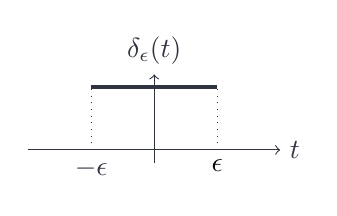
\begin{tikzpicture}[scale=0.8, baseline={(current bounding box.center)}]
      \pgfmathsetmacro{\eps}{1} % for plotting purposes, assume epsilon=1
      \pgfmathsetmacro{\hgt}{1/(\eps)}
      % Axes
      \draw[->, gray3] (-2,0) -- (2,0) node[right] {$t$};
      \draw[->, gray3] (0,-0.2) -- (0,1.2) node[above] {$\delta_{\epsilon}(t)$};
      % Plot: horizontal line over (-eps,eps) at height hgt
      \draw[line width=1.2pt, gray3] (-\eps,\hgt) -- (\eps,\hgt);
      % Dotted vertical lines showing the jump edges
      \draw[dotted, gray3] (-\eps,0) -- (-\eps,\hgt);
      \draw[dotted, gray3] (\eps,0) -- (\eps,\hgt);

      \node[below, gray3] at (-\eps,0) {$-\epsilon$};
      \node[below] at (\eps,0) {$\epsilon$};
    \end{tikzpicture}
     &
    \delta_{\epsilon}(t)=
    \begin{cases}
      \dfrac{1}{2\epsilon} & \text{if } t \in  [-\epsilon,\epsilon], \\
      0                    & \text{otherwise.}
    \end{cases}
  \end{array}
$$
This function creates a rectangular pulse with the following propertites:
$$\textbf{Height: } \frac{1}{2 \varepsilon} \quad \textbf{Width: } 2\varepsilon \quad \textbf{Area: } 1\;\text{(always)}$$
As $\varepsilon$ approaches 0, the function becomes infinitely tall and thin, but the area remains 1. This limit defines the Dirac Delta Function:
$$\delta(t) = \lim_{\varepsilon \to 0+} \{\delta_{\varepsilon}(t)\}$$
\textbf{Properties of the Dirac Delta Function:}
\begin{align*}
   & \delta(t) = 0 \text{ for } t \neq 0                     \\
   & \int_{-\infty}^{\infty} \delta(t)\, dt = 1              \\
   & \int_{-\infty}^{\infty} \delta(t-t_0)f(t)\; dt = f(t_0)
\end{align*}
The Laplace Transform of the Dirac Delta Function is:
$$L\{\delta(t-t_0)\} = \int_{0}^{\infty} e^{-st}\delta(t - t_0) \; dt = \int_{-\infty}^{\infty} e^{-st}\delta(t-t_0) \; dt = e^{-st_0} \quad \text{for} \; \; t_0 > 0$$

\subsubsection{Examples}
\begin{examplebox}[ : Solve the following initial value problem which governs the behavious of an RLC circuit]
  \scriptsize
  \begin{align*}
    LQ'' + RQ' + \frac{Q}{C} & = V_0 \delta(t-a) \\
    Q(0)                     & = 0               \\
    Q'(0)                    & = 0
  \end{align*}
  Where $a,L,R,C,V_0$ are all positive constans and $4L > R^2C$. \\
  Note that the applied voltage corresponds to an impulse of stength $V_0$ at $t=a$ \\
  We note that:
  \begin{align*}
    L\{Q''\} = s^2 L\{Q\} - sQ(0) - Q'(0) & = s^2 L\{Q\} \\
    L\{Q'\} = sL\{Q\} - Q(0)              & = sL\{Q\}    \\
    L\{\delta(t-a)\} = e^{-st_0}          & = e^{-as}
  \end{align*}
  Thus:
  $$L\{LQ'' + RQ' + \frac{Q}{C} = V_0 \delta(t-a)\} = Ls^2L\{Q\} + RsL\{Q\} + \frac{1}{C}L\{Q\} = V_0 e^{-as}$$
  Grouping terms:
  $$L\{Q\}(Ls^2 + Rs + \frac{1}{C}) = V_0 e^{-as}$$
  Hence:
  $$L\{Q\} = V_0 e^{-as} \cdot \frac{1}{Ls^2 + Rs + \frac{1}{C}}$$
  Removing the $L$ from the denominator gives:
  \begin{align*}
    L\{Q\} & = \frac{V_0}{L}e^{-as} \cdot \frac{1}{s^2 + \frac{R}{L}s + \frac{1}{LC}} \\
           & =\frac{V_0}{L}\cdot \frac{e^{-as}}{s^2 + \frac{R}{L}s + \frac{1}{LC}}
  \end{align*}
  We notice that:
  \begin{align*}
    (s+\frac{R}{2L})^2 & = s^2 + s \frac{2R}{2L} + \frac{R^2}{4L^2} \\
                       & = s^2 + \frac{R}{L}s + \frac{R^2}{4L^2}
  \end{align*}
  So that:
  $$L\{Q\} = \frac{V_0}{L} \frac{e^{-as}}{(s+\frac{R}{2L})^2 - \frac{R^2}{4L^2} + \frac{1}{LC}}$$
  Rewriting with $\alpha = \frac{R}{2L}$ and $\beta = \frac{1}{LC} - \frac{R^2}{4L^2}$
  $$L\{Q\} = \frac{V_0}{L} \frac{e^{-as}}{(s+\alpha)^2 + \beta}$$

  We also note that:
  $$L\{\sin(\beta t)\} = \frac{\beta}{s^2 + B^2} \xRightarrow{\text{First Shift Theorem}} L\{e^{-as} \sin(\beta t)\} = \frac{B}{(s+a)^2 + \beta^2}$$
  Or,
  $$L^{-1} \left\{\frac{B}{(s+a)^2 + \beta^2}\right\} = e^{-at}\sin(\beta t)$$
  We can also write:
  $$L^{-1}\{F(s)\} = f(t)$$
  Notice that:
  $$f(t-a) = e^{-a(t-a)} \sin(\beta [t-a])$$
  Applying the Second Shift Theorem gives:
  $$L^{-1}\{e^{-a} F(s)\} = f(t-a)H(t-a)$$
  $$L^{-1} \left\{e^{-as}\frac{\beta}{(s+a)^2 + \beta^2}\right\} = e^{-a(t-a)}\sin(\beta[t-a])H(t-a)$$
  Thus:
  \begin{align*}
    Q(t) & = \frac{V_0}{L\beta} e^{-a(t-a)}\sin(\beta[t-a])H(t-a)                                \\
         & = \begin{cases}
               0                                                     & \text{for}\;\; 0 \leq t < a \\
               \dfrac{V_0}{L\beta} e^{-a(t-a)}\sin(\beta[t-a])H(t-a) & \text{for}\;\; t > a
             \end{cases}
  \end{align*}
  \normalsize
\end{examplebox}
\pagebreak
\subsection{Differentiation of the Laplace Transform}
Suppose $f(t), t \geq 0$ satisfies the conditions of the existence theorem so
that its Laplace Transform ($F(s))$ exists for some $s > k$. Then:
$$F'(s) = \diff{}{s} \left\{ \int_0^\infty e^{-st}f(t)\; dt \right\} = \int_0^\infty \pdiff{}{s}\{e^{-st}f(t) \; dt\}$$
We are allowed to bring the derivative inside the integral provided the conditions of the existence theorem are satisfied, hence:
$$F'(s) = -\int_0^\infty e^{-st}\{tf(t)\}\; dt = -L\{tf(t)\}$$
so that,
$$L\{tf(t)\} = -F'(s)$$
We can sometimes use this to calculate transforms and inverse transforms. For example:
$$L\{t\} = L\{t \cdot 1\} = - \diff{}{s}L\{1\} = -\diff{}{s}\left(\frac{1}{s}\right) = \frac{1}{s^2}$$

\subsection{The Convolution Function}
Let $f(t), g(t)$ be two functions. Define the Convolution function
$$(f \star g)(t) = \int_0^t f(t-\tau)g(\tau) \; d\tau$$
Where $\tau$ is integrated over the interval $[0,t]$.  The Convolution is:
\begin{align*}
  \textbf{Commutative:}         & f \star g = g \star f                     \\
  \textbf{Associative:}         & f \star (g \star h) = (f \star g) \star h \\
  \textbf{Distruibutive:}       & f \star (g + h) = f \star g + f \star h   \\
  \textbf{Multiplication by 0:} & = f \star (ag) = a(f \star g)
\end{align*}

\begin{theorembox}
  Let $f(t)$ and $g(t)$ have Laplace Transforms $F(s)$ and $G(s)$ respectively defined for $s > k \geq 04$. Then
  $$L\{f \star g\} = F(s)G(s), \quad s > k$$
\end{theorembox}

\begin{proofbox}
  Write \( F(s) = \int_{0}^{\infty} e^{-s\sigma} f(\sigma) \, d\sigma \) and \( G(s) = \int_{0}^{\infty} e^{-s\tau} g(\tau) \, d\tau \).
  Then:
  \begin{align*}
    F(s)G(s) & = \left\{ \int_{0}^{\infty} e^{-s\sigma} f(\sigma) \, d\sigma \right\} \left\{ \int_{0}^{\infty} e^{-s\tau} g(\tau) \, d\tau \right\} \\
             & = \int_{0}^{\infty} e^{-s\tau} g(\tau) \left\{ \int_{0}^{\infty} e^{-s\sigma} f(\sigma) \, d\sigma \right\} d\tau                     \\
             & = \int_{0}^{\infty} g(\tau) \left\{ \int_{0}^{\infty} e^{-s(\sigma+\tau)} f(\sigma) \, d\sigma \right\} d\tau.                        \\
  \end{align*}
\end{proofbox}

\pagebreak

\section{Line Integrals}
\begin{minipage}{0.69\textwidth}
  Consider a mass which undergoes a displacement, $\boldsymbol{d}$, under a constant force $\boldsymbol{F}$. Define the work, $\boldsymbol{W}$, done by $\boldsymbol{F}$ to be the magnitude of the force multiplied by the distance moved in the direction of the force.
  Inspecting the diagram, we see that work done $\boldsymbol{W}$ is given by the dot product of $\boldsymbol{F}$ and $\boldsymbol{d}$:
  $$W = |F| \cdot |d| \cdot \cos(\theta) = \boldsymbol{F} \cdot \boldsymbol{d}$$
  Now, lets suppose $F$ is not constant:
\end{minipage}
\begin{minipage}{0.3\textwidth}
  \begin{center}
    \begin{tikzpicture}[scale= 0.8, baseline={(-3,-1)}] % Added xshift=3cm
      % Draw displacement vector
      \draw[->, thick] (0,0) -- (4,0) node[right] {$\boldsymbol{d}$};

      % Draw force vector
      \draw[->, thick] (0,0) -- (3,2) node[above] {$\boldsymbol{F}$};

      % Draw arc for angle
      \draw (1.3,0) arc (0:33:1.3);

      % Label angle
      \node at (0.85,0.3) {$\theta$};

      % Draw dotted projection line
      \draw[dotted] (3,2) -- (3,0);
    \end{tikzpicture}
  \end{center}

\end{minipage}




$$F = F(x,y,z) = F(r) = r(x,y,z)$$
Suppose further, that $F$ acts for a time $t_1 \leq t \leq t_2$ and the path of the object in this time interval is given by a curve $\mathcal{C}$ defined by:
$$\mathbf{r} = \left(x(t), y(t), z(t) \right) \quad t \in [t_1, t_2]$$
But how do we calculate the work done by $F$ along $\mathcal{C}?$
\begin{center}
  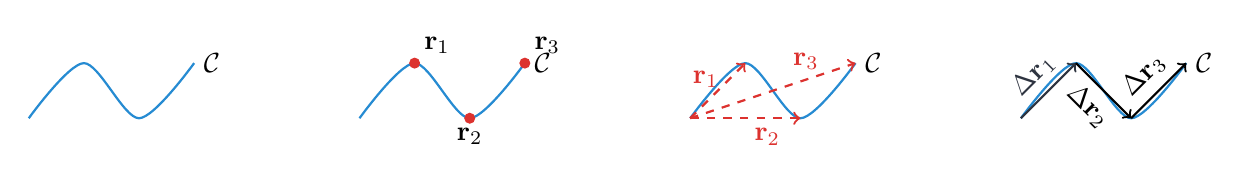
\begin{tikzpicture}[scale=0.7]
    % First graph - just curve C
    \begin{scope}
      \draw[thick, custom_blue] plot [smooth] coordinates {(0,0) (1,1) (2,0) (3,1)};
      \node[right] at (3,1) {$\mathcal{C}$};
    \end{scope}

    \begin{scope}[xshift=6cm]
      \draw[thick, custom_blue] plot [smooth] coordinates {(0,0) (1,1) (2,0) (3,1)};
      \node[right] at (3,1) {$\mathcal{C}$};

      \fill[custom_red] (1,1) circle (0.1);
      \fill[custom_red] (2,0) circle (0.1);
      \fill[custom_red] (3,1) circle (0.1);

      % Add labels for points
      \node[above right] at (1,1) {$\mathbf{r}_1$};
      \node[below] at (2,0) {$\mathbf{r}_2$};
      \node[above right] at (3,1) {$\mathbf{r}_3$};
    \end{scope}

    % Second graph - curve C and position vectors r  
    \begin{scope}[xshift=12cm]
      \draw[thick, custom_blue] plot [smooth] coordinates {(0,0) (1,1) (2,0) (3,1)};
      \node[right] at (3,1) {$\mathcal{C}$};
      \draw[->,dashed, custom_red, thick] (0,0) -- (1,1) node[pos=0.7, left] {$\mathbf{r}_1$};
      \draw[->, dashed, custom_red, thick] (0,0) -- (2,0) node[pos=0.7, below] {$\mathbf{r}_2$};
      \draw[->, dashed, custom_red, thick] (0,0) -- (3,1) node[pos=0.7, above] {$\mathbf{r}_3$};
    \end{scope}

    % Third graph - curve C, position vectors r, and displacement vectors Δr
    \begin{scope}[xshift=18cm]
      \draw[thick, custom_blue] plot [smooth] coordinates {(0,0) (1,1) (2,0) (3,1)};
      \node[right] at (3,1) {$\mathcal{C}$};

      \draw[->, thick, gray3] (0,0) -- (1,1) node[midway, sloped, above] {$\Delta \mathbf{r}_1$};
      \draw[->, thick] (1,1) -- (2,0) node[midway, sloped, below] {$\Delta \mathbf{r}_2$};
      \draw[->, thick] (2,0) -- (3,1) node[midway, sloped, above] {$\Delta \mathbf{r}_3$};
    \end{scope}
  \end{tikzpicture}
\end{center}
As seen as the diagram above, we can divide $\mathcal{C}$ into a a large number $N-1$ of small segment of $\Delta \mathbf{r}_i$ and approximate the work done by $F$ along $\mathcal{C}$ by the sum of the work done along each segment:
$$W \approx \sum_{i=1}^{N-1} F(\mathbf{r}_i) \cdot \Delta \mathbf{r}_i$$

\subsection{The Line Integral}
Taking the limit $N \to \infty$
$$W = \lim_{N \to \infty} \left\{ \sum_{i=1}^{N-1} F(\mathbf{r}_i) \cdot \Delta \mathbf{r}_i \right\}$$
This limit is called the \textbf{line integral} of $F$ along $\mathcal{C}$ and is denoted by $\int_{\mathcal{C}} F(r)\cdot d\mathbf{r}$, that is:
$$\int_{\mathcal{C}} F(r) \cdot dr = \lim_{N \to \infty} \left\{ \sum_{i=1}^{N-1}F(r_i)\cdot \Delta r_i \right\}$$
Since $r = r(t)$ we can calculate the line integral as:
$$\int_{\mathcal{C}} F(r) \cdot dr = \int_{t_1}^{t_2} F(r(t)) \cdot \diff{r}{t} \; dt$$
In general, $t$, may be any variable that parametrizes (traces out) the curve $\mathcal{C}$. Then $dr = \diff{r}{t} \; dt$ is the tangent vector to $\mathcal{C}$ at the point $r(t)$. We call $\mathcal{C}$ the \textbf{path of integration} and $r(t_1)$ the initial point, $r(t_2)$ the \textbf{terminal point}. $\mathcal{C}$ is now \textbf{oriented} from $r(t_1)$ to $r(t_2)$. \\
The direction for $r(t_1) \to r(t_2)$, in which $t$ increases, is called the \textbf{positive direction} of $\mathcal{C}$, we indicate this by an arrow on $\mathcal{C}$.

\begin{center}
  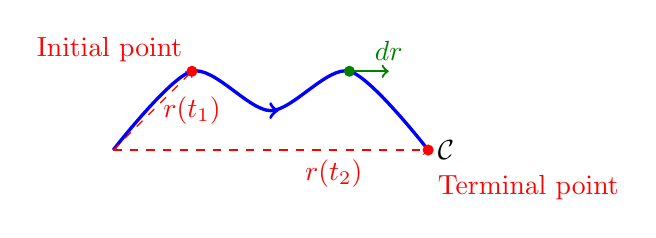
\begin{tikzpicture}
    % Draw curve C
    \draw[very thick, blue] plot [smooth] coordinates {(0,0) (1,1) (2,0.5) (3,1) (4,0)};
    \draw[->, very thick, blue] plot [smooth] coordinates {(2,0.5) (2,0.5) (2.1,0.5)};
    \node[right] at (4,0) {$\mathcal{C}$};

    % Draw position vectors 
    \draw[->, dashed, red] (0,0) -- (1,1) node[pos=1, below=0.2cm] {$r(t_1)$};
    \draw[->, dashed, red] (0,0) -- (4,0) node[pos=0.7, below] {$r(t_2)$};

    % Add red dots at vector endpoints
    \fill[red] (1,1) circle (2pt);
    \fill[red] (4,0) circle (2pt);

    % Draw tangent vector at a point
    \draw[->, thick,  green!50!black] (3,1) -- (3.5,1) node[above] {$dr$};
    \fill[green!50!black] (3,1) circle (2pt);

    % Label points
    \node[red, above left] at (1,1) {Initial point};
    \node[red, below right] at (4,-0.2) {Terminal point};
  \end{tikzpicture}
\end{center}
If $r(t_1) = r(t_2)$ then $\mathcal{C}$ is a \textbf{closed curve} and the line integral is denoted by:
$$\oint_{\mathcal{C}} F(r) \cdot dr$$
The line integral of $F$ alonged a closed curve $\mathcal{C}$ is called the \textbf{circulation} of $F$ around $\mathcal{C}$.

\pagebreak
\subsubsection{Examples}
\begin{examplebox}[: For a time period $0 \leq t \leq 1$, a particle moves along a trajectory defined by $\mathcal{C} = x = t, y = t, z = 2t^2$, a force $F(r) = (y,x,z)$ acts. Calculate work done.]
  We have:
  \begin{align*}
    \mathbf{r}           & = (t,t,2t^2) \\
    \diff{\mathbf{r}}{t} & = (1,1,4t)   \\
    F(\mathbf{r})        & = (t,t,2t^2)
  \end{align*}
  The work done is:
  \begin{align*}
    \int_{\mathcal{C}} F(r) \cdot dr & = \int_{0}^{1} (t,t,2t^2) \cdot (1,1,4t) \; dt \\
                                     & = \int_{0}^{1} (t + t + 8t^3) \; dt            \\
                                     & = \int_{0}^{1} (2t + 8t^3) \; dt               \\
                                     & = \left[t^2 + 2t^4\right]_0^1                  \\
                                     & = 1 + 2                                        \\
                                     & = 3
  \end{align*}
\end{examplebox}

\begin{examplebox}[Evaluate $\int_{\mathcal{C}} F(r) \cdot dr$ for $F(r) = (y+z, x+z, x+y)$, where $\mathcal{C}$ is the line segment joinint $A:(-2,2,-3) \to B(2,4,6)$ ]
  We can parametrize any straight line in three dimensions by writing:
  $$x = c_1t + c_2 \quad y=c_3t + c_4 \quad z = c_5t + c_6$$
  where the $c_i$ are constants. \\
  We can take $t = 0$ to correspond with $A$ and $t = 1$ to correspond with $B$. \\
  Hence setting $t = 0$ gives:
  $$c_2 = -2 \quad  c_4 = 2 \quad c_6 = -3$$
  Setting $t = 1$ gives:
  $c_1 + c_2 = 2 \quad c_3 + c_4 = 4 \quad c_5 + c_6 = 6$ so that:
  $$c_1 = 4 \quad c_3 = 2 \quad c_5 = 9$$
  Hence, the required line is given by:
  $$x = 4t - 2 \quad y = 2t + 2 \quad z = 9t - 3$$
  We have:
  \begin{align*}
    \int_\mathcal{C} F(r) \cdot dr & = \int_0^1 (11t - 1, 13t -5,6t) \cdot \diff{}{t}(4t-2, 2t+2, 9t-3) \; dt \\
                                   & = \int_0^1 (11t - 1, 13t -5,6t) \cdot (4,2,9) \; dt                      \\
                                   & = \int_0^1 (44t - 4 + 26t - 10 + 54t) \; dt                              \\
                                   & = \int_0^1 (124t - 12) \; dt                                             \\
                                   & = \left[62t^2 - 14t\right]_0^1                                           \\
                                   & = 48
  \end{align*}
\end{examplebox}

\begin{examplebox}[Find the circulation of the vector $F = (y, -x, 0)$ around the unit circle $\mathcal{C} = x^2 + y^2 = 1$, $z=0$, taken in an anti-clockwise direction]
  We can parametrize the unit circle by setting $x,y$ and $z$ to:
  $$x = \cos(t) \quad y = \sin(t) \quad z = 0$$
  We can write the position vector as:
  $$\mathbf{r} = (\cos(t), \sin(t), 0)$$
  The tangent vector is:
  $$\diff{\mathbf{r}}{t} = (-\sin(t), \cos(t), 0)$$
  The force vector is:
  $$F(\mathbf{r}) = (\sin(t), -\cos(t), 0)$$
  The circulation is:
  \begin{align}
    \oint_{\mathcal{C}} F(r) \cdot dr & = \int_0^{2\pi} (\sin(t), -\cos(t), 0) \cdot (-\sin(t), \cos(t), 0) \; dt \\
                                      & = \int_0^{2\pi} -\sin^2(t) - \cos^2(t) \; dt                              \\
                                      & = -\int_0^{2\pi} (\sin^2(t) + \cos^2(t)) \; dt                            \\
                                      & = -\int_0^{2\pi} 1 \; dt                                                  \\
                                      & = -\left[t\right]_0^{2\pi}                                                \\
                                      & = -2\pi
  \end{align}
\end{examplebox}


% Add the other examples here
\subsection{Convervative Vector Fields}
A vector field $F$ is called \textbf{conservative} if the line integral of $F$ along any closed curve $\mathcal{C}$ is zero, that is:
$$\oint_{\mathcal{C}} F(r) \cdot dr = 0$$
An equivalent definition is that $F$ is conservative if the line integral of $F$ depends only on the end points of the curce, not on the path taken, so that:
$$\int_{\mathcal{C}_1} F(r) \cdot dr = \int_{\mathcal{C}_2} F(r)\cdot dr$$
Where $\mathcal{C}_1$ and $\mathcal{C}_2$ are two curves with the same initial and terminal points but different paths.

\begin{center}
  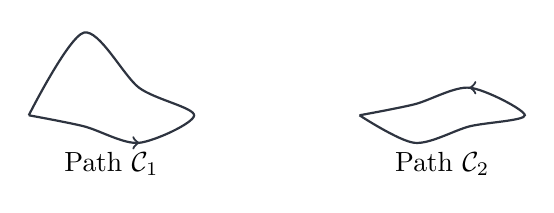
\begin{tikzpicture}[scale=0.7]
    % First path - now closed
    \begin{scope}
      \draw[thick, gray3] plot [smooth] coordinates {(0,0) (1,1.5) (2,0.5) (3,0) (2,-0.5) (1,-0.2) (0,0)};
      \draw[->, thick, gray3] plot [smooth] coordinates {(2,-0.5) (2,-0.5) (2.01, -0.5)};
      \node[below] at (1.5,-0.5) {Path $\mathcal{C}_1$};
    \end{scope}

    % Second path - now closed (5 units to the right)
    \begin{scope}[xshift=6cm]
      \draw[thick, gray3] plot [smooth] coordinates {(0,0) (1,-0.5) (2,-0.2) (3,0) (2,0.5) (1,0.2) (0,0)};
      \draw[->, thick, gray3] plot [smooth] coordinates {(2,0.5) (2,0.5) (1.99, 0.5)}; % Fix this arrow
      \node[below] at (1.5,-0.5) {Path $\mathcal{C}_2$};
    \end{scope}
  \end{tikzpicture}
\end{center}
Consider two curves, $\mathcal{C}_1$ and $\mathcal{C}_2$, that start at $A$ and end at $B$. Let $\mathcal{C}$ be the closed curve that starts at $A$ follows the curve $\mathcal{C}_1$  and then follows $\mathcal{C}_2$ in the reverse direction to $B$. Then:
\begin{align*}
  \oint_{\mathcal{C}} F(r) \cdot dr & = \int_{A\mathcal{C}_1}^B F(r) \cdot dr + \int_{B\mathcal{C}_2}^A F(r) \cdot dr     \\
                                    & = \int_{A\mathcal{C}_1}^B F(r) \cdot dr - \int_{A\mathcal{C}_2}^B F(r) \cdot dr = 0
\end{align*}
Thus:
$$\oint_{\mathcal{C}} F(r) \cdot dr = 0 \Rightarrow \int_{A\mathcal{C}_1}^B F(r) \cdot dr = \int_{A\mathcal{C}_2}^B F(r) \cdot dr$$
\subsubsection{Examples}
\begin{examplebox}[By considering the line integral of $F = (y, x^2 -x, 0)$ around the square $C$ in the $x,y$ plane connecting for point $(0, 0, 0), (1, 0, 0), (1, 1, 0), (0, 1, 0)$, show that $F$ cannot be conservative. ]
  Split $\mathcal{C}$ into four segments, $\mathcal{C}_1, \mathcal{C}_2, \mathcal{C}_3, \mathcal{C}_4$ and calculate the line integral of $F$ along each segment.
  \begin{center}
    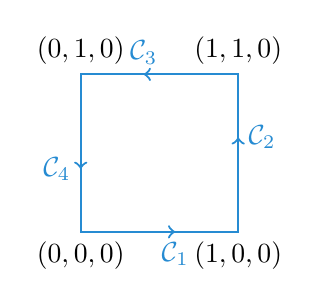
\begin{tikzpicture}[scale=2]
      % Draw the square
      \draw[thick, custom_blue] (0,0) -- (1,0) -- (1,1) -- (0,1) -- cycle;
      % Add arrows for direction
      \draw[->, thick, custom_blue] (0.5,0) -- (0.6,0) node[below] {$\mathcal{C}_1$};
      \draw[->, thick, custom_blue] (1,0.5) -- (1,0.6) node[right] {$\mathcal{C}_2$};
      \draw[->, thick, custom_blue] (0.5,1) -- (0.4,1) node[above] {$\mathcal{C}_3$};
      \draw[->, thick, custom_blue] (0,0.5) -- (0,0.4) node[left] {$\mathcal{C}_4$};
      % Label vertices
      \node[below] at (0,0) {$(0,0,0)$};
      \node[below] at (1,0) {$(1,0,0)$};
      \node[above] at (1,1) {$(1,1,0)$};
      \node[above] at (0,1) {$(0,1,0)$};
    \end{tikzpicture}
  \end{center}
  We have:
  \begin{align*}
    \int_{\mathcal{C}_1} F(r) \cdot dr & = \int_{0}^{1} (0, t^2 - t, 0) \cdot (1, 0, 0) \; dt = 0                                                                                    \\
    \int_{\mathcal{C}_2} F(r) \cdot dr & = \int_{0}^{1} (t, 1 - t, 0) \cdot (0, 1, 0) \; dt = \int_{0}^{1} (1-t) \; dt = [t - \frac{t^2}{2}]_{0}^{1} = 1 - \frac{1}{2} = \frac{1}{2} \\
    \int_{\mathcal{C}_3} F(r) \cdot dr & = \int_{0}^{1} (1, (1-t)^2-(1-t), 0) \cdot (-1, 0, 0) \; dt = \int_{0}^{1} -1 \; dt = -1                                                    \\
    \int_{\mathcal{C}_4} F(r) \cdot dr & = \int_{0}^{1} (1-t, 0, 0) \cdot (0, -1, 0) \; dt = 0
  \end{align*}
  Hence:
  $$\oint_{\mathcal{C}} F(r) \cdot dr = \int_{\mathcal{C}_1} F(r) \cdot dr + \int_{\mathcal{C}_2} F(r) \cdot dr + \int_{\mathcal{C}_3} F(r) \cdot dr + \int_{\mathcal{C}_4} F(r) \cdot dr = 0 + \frac{1}{2} + (-1) + 0 = -\frac{1}{2} \neq 0$$
  Thus, $F$ is not conservative.
\end{examplebox}

\section{Gradient, Divergence and Curl}
\subsection{Gradient}
\begin{definitionbox}
  The gradient of a differentiable function $\phi(x,y,z)$ is the vector field:
  $$\text{grad}(\phi) =  \nabla \phi = \diff{\phi}{x} \hat{i} + \diff{\phi}{y} \hat{j} + \diff{\phi}{z} \hat{k}$$
\end{definitionbox}

\begin{center}
  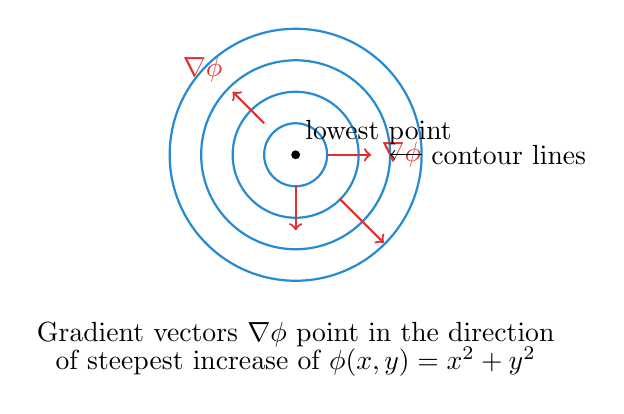
\begin{tikzpicture}[scale=0.8]
    % Draw hill contours (representing a function like z = x^2 + y^2)
    \draw[thick, custom_blue] (0,0) circle (0.5);
    \draw[thick, custom_blue] (0,0) circle (1);
    \draw[thick, custom_blue] (0,0) circle (1.5);
    \draw[thick, custom_blue] (0,0) circle (2);

    % Draw gradient vectors - pointing outward from the center
    \draw[->, thick, custom_red] (0.5,0) -- (1.2,0) node[right] {$\nabla\phi$};
    \draw[->, thick, custom_red] (0,-0.5) -- (0,-1.2);
    \draw[->, thick, custom_red] (-0.5,0.5) -- (-1,1) node[above left] {$\nabla\phi$};
    \draw[->, thick, custom_red] (0.7,-0.7) -- (1.4,-1.4);

    % Label lowest point and add explanation
    \fill (0,0) circle (2pt) node[above right] {lowest point};
    \node[below] at (0,-2.5) {Gradient vectors $\nabla\phi$ point in the direction};
    \node[below] at (0,-2.9) {of steepest increase of $\phi(x,y)=x^2+y^2$};

    % Label contour lines
    \node[right] at (2,0) {contour lines};
    \draw[->] (2,0) -- (1.5,0);
  \end{tikzpicture}

  \hspace{1cm}
  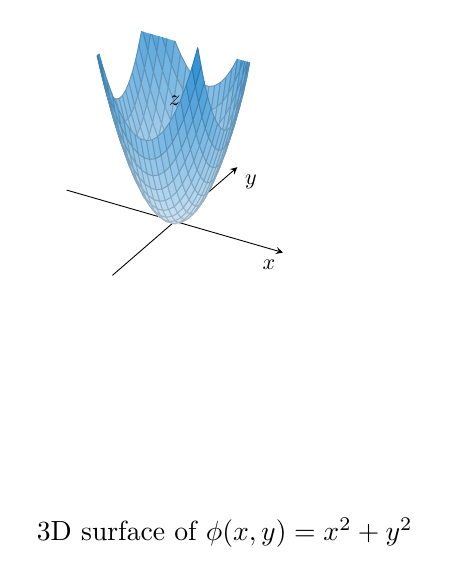
\begin{tikzpicture}[scale=0.8]
    % 3D plot using pgfplots
    \begin{axis}[
        width=7cm,
        height=6cm,
        view={30}{30},
        axis lines=center,
        xlabel=$x$,
        ylabel=$y$,
        zlabel=$z$,
        xlabel style={anchor=north east},
        ylabel style={anchor=north west},
        zlabel style={anchor=south},
        xmin=-2, xmax=2,
        ymin=-2, ymax=2,
        zmin=0, zmax=4,
        xtick=\empty,
        ytick=\empty,
        ztick=\empty,
        axis equal,
        colormap={paraboloid}{color(0)=(custom_blue!20) color(1)=(custom_blue)},
      ]
      % 3D paraboloid surface
      \addplot3[
        surf,
        domain=-2:2,
        domain y=-2:2,
        samples=20,
        samples y=20,
      ] {x*x + y*y};


    \end{axis}

    \node[below] at (3.5,-3.2) {3D surface of $\phi(x,y) = x^2 + y^2$};
  \end{tikzpicture}
\end{center}



\pagebreak

\subsubsection{The Directional Derivative}
\noindent\begin{minipage}{0.8\textwidth}
  Consider a differentiable function $\phi(x,y,z)$ at a point $P$, with a position vector $\vec{r}_0$.  \\
  We want to find the rate of change of $\phi$ as we move from $P$ in the direction of $\hat{\mathbf{n}}$. \\
  Consider the line segment $L$ through $P$ in the direction of $\hat{\mathbf{n}}$ \\
  Let $Q(s)$ be the point on $L$ a distance $s$ from $P$ \\
  Define the \textbf{Directional Derivative} of $\phi(x,y,z)$ in the direction of $\hat{\mathbf{n}}$ by:
\end{minipage}
\begin{minipage}{0.2\textwidth}
  \begin{center}
    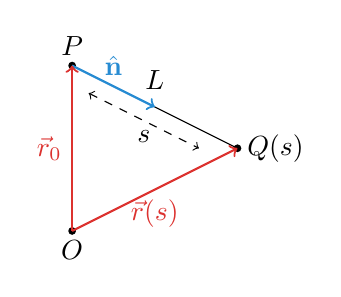
\begin{tikzpicture}[scale=0.7]
      \fill(0,3) circle (2pt) node[above] {$P$};
      \fill(0,0) circle (2pt) node[below] {$O$};
      \fill(3,1.5) circle (2pt) node[right] {$Q(s)$};



      \draw[-, black] (0,3) -- (3,1.5) node[midway, above=0.1cm] {$L$};

      \draw[<->, dashed, black] (0.3,2.5) -- (2.3,1.5) node[below, midway] {$s$};
      \draw[->, thick, custom_blue] (0,3) -- (1.5,2.25) node[midway, above] {$\hat{\mathbf{n}}$};

      \draw[->, thick, custom_red] (0,0) -- (0,3) node[midway, left] {$\vec{r}_0$};
      \draw[->, thick, custom_red] (0,0) -- (3,1.5) node[midway, below] {$\vec{r}(s)$};

    \end{tikzpicture}
  \end{center}
\end{minipage}

$$D_{\hat{\mathbf{n}}} \phi = \lim_{s \to 0} \frac{\phi(Q(s)) - \phi(P)}{s}$$
That is, as $s$ gets smaller and smaller we get a better and better approximation of
With $L$ described by $r(s) = x(s) \hat{i} + y(s) \hat{j} + z(s) \hat{k}$, we have:
\begin{align*}
  D_{\hat{\mathbf{n}}} \phi & = \lim_{s \to 0} \frac{\phi(r(s)) - \phi(r(0))}{s}                         \\
                            & = \lim_{s \to 0} \frac{\phi(x(s), y(s), z(s)) - \phi(x(0), y(0), z(0))}{s} \\
                            & = \diff{\phi}{s}
\end{align*}
Writing $\hat{\mathbf{n}} = (n_1, n_2, n_3)$ and using the chain rule:
\begin{align}
  D_{\hat{\mathbf{n}}} \phi & = \diff{\phi}{s} = \diff{\phi}{x} \diff{x}{s} + \diff{\phi}{y} \diff{y}{s} + \diff{\phi}{z} \diff{z}{s} \nonumber \\
                            & = \diff{\phi}{x} n_1 + \diff{\phi}{y} n_2 + \diff{\phi}{z} n_3
\end{align}
and so with $|\hat{\mathbf{n}}| = 1$, we have:
$$D_{\hat{\mathbf{n}}} \phi = \hat{\mathbf{n}} \cdot \nabla \phi $$

\begin{examplebox}[Find the directional derivative of $\phi(x,y,z) = 2x^2 + 3y^2 + z^2$ at the point
    $P: : (2,1,3)$ in the direction of the vector $\vec{a} = \hat{i} - 2\hat{k}$]
  First we calculate the gradient of $\phi$:
  $$\nabla \phi = \diff{}{x}(2x^2) \hat{i} + \diff{}{y}(3y^2) \hat{j} + \diff{}{z}(z^2) \hat{k} = 4x \hat{i} + 6y \hat{j} + 2z \hat{k}$$
  At $P : (2,1,3)$, the gradient is evaluated as
  $$\nabla \phi = 4(2) \hat{i} + 6(1) \hat{j} + 2(3) \hat{k} = 8 \hat{i} + 6 \hat{j} + 6 \hat{k}$$
  Since $\vec{a}$ is not a unit vector, i.e. $|\vec{a}| \neq 1$, we need to normalize it to get a unit vector $\hat{\mathbf{n}}$:
  $$\hat{\mathbf{n}} = \frac{\vec{a}}{|\vec{a}|} = \frac{\hat{i} - 2\hat{k}}{\sqrt{1 + 4}} = \frac{\hat{i} - 2\hat{k}}{\sqrt{5}}$$
  The directional derivative is then:
  $$D_{\hat{\mathbf{n}}} \phi \mid_P = \hat{\mathbf{n}} \cdot \nabla \phi\mid_P = \frac{\hat{i} - 2\hat{k} \cdot (8\hat{i} + 6\hat{j} + 6\hat{k})}{\sqrt{5}} = \frac{8 - 12}{\sqrt{5}} = -\frac{4}{\sqrt{5}}$$
  \emph{Note:} The fact the directional derivative is negative indicates that $\phi$ decreases in the direction of $\vec{a}$.
\end{examplebox}


\end{document}
